%**************************************************%
% Author     : Fatih Selim Yakar                   %
% ID         : 161044054                           %
% Title      : Systems Programming HW5 Report      %
% Instructor : Erchan Aptoula                      %
%**************************************************%

\documentclass{article}

\usepackage[utf8]{inputenc}
\usepackage[margin=1in]{geometry}
\usepackage[titletoc,title]{appendix}

\usepackage{graphicx}
\graphicspath{ {.} }

\usepackage{minted}
\usemintedstyle{borland}

\usepackage{biblatex}
\addbibresource{references.bib}

% Title content
\title{\textbf{CSE344 System Programming HW5 Report}}
\begin{document}

\maketitle

% Center
\begin{center}
    \textbf{Student:}Fatih Selim YAKAR \\
    \textbf{Student No:}161044054 \\
    \textbf{Instructor:}Erchan APTOULA
\end{center}

\newpage

%Overview
\section{Overview}
\par{In this assignment, I simulated the synchronization and exchange between an indefinite number of florists and main threads through pthread tools. The context was as follows: There was an input file, and in the first part of this input file, there were the names of the florists, their locations, the speed of delivery, and the list of flowers in their hands. In the second part, there were the clients to be assigned to the florists, their locations and the desired flower. From us, with the main thread procedure, it was to direct the clients to a florist closest to him and with the flower he wanted. Of these two structs, I created global arrays, so that all threads were able to reach. I created mutex for the number of florists for critical sections. For some cases, I solved the wait by creating a condition variable as many as the number of florists. For finishing in the Ctrl-c state and the nominal state, I used condition variables first. In any case, I freed all the resources while the program was over. You can find the details below.}

% Synchronization Problem Between Threads
\section{Synchronization Problem Between Threads}
\par{In case of this homework, there are main thread also there are florist threads. Threads have to work in parallel among themselves. On the other hand, in the critical section, it is necessary to add a client to the queues of each florist with the main thread and to get a client from the queues by the florist threads.}

% Providing critical section
\subsection{Providing critical section}
\par{I used mutex to provide the critical section. If I tried to do this for all threads with a single mutex, not all threads would work at the same time. I created a separate mutex for each florist to ensure that all threads can work in parallel, and while adding a queueya client to the main thread, I locked the necessary florist's mutex and performed the necessary operation and unlocked it after doing the operation. Likewise, within florist, each florist made the process of bringing and delivering its own flowers in the lock and unlock of its mutex.}


\subsection{Waiting with condition variables for queues}
\par{I created a client queue for each florist. When these queues are full, the main thread should not add customers to the queue and the florist should not receive customers from the queue when the queue is empty. So in these cases, he should wait for it to fill up or empty. Since I created each queue as much as the maximum number of clients, I did not use a condition variable related to its stuffing. But since the florist should wait if the queue is empty, I have defined the condition variable as many as the number of florists. I did pthread cond signal when adding client to main thread queue. And in the florist thread I made pthread cond wait if the size of the queue was zero so I solved the sync issue in the queues.}


\subsection{Waiting with mutex to finish}
\par{When all threads are finished, that is, when the total number of clients is delivered, the threads must close themselves. Whichever of the florist threads ends the process, the thread that ends the process awakens the other threads sending pthread cond signals to the remaining thread's condition variables, waking them from sleep, and ending them. Thus, all threads end properly.}


\section{In Case Of SIGINT(ctrl-c)}
\par{Unexpected termination of the program (that is, SIGINT signal coming) was designed as follows: Firstly, I activated a thread handle function with sigaction. But right after that, I blocked the SIGINT signal from the beginning of the main function to the end of the thread where the threads were joined. In the meantime, I checked if the SIGINT signal was coming in the threads while it was blocked with the sigpending function. In the case of his arrival, I quit instantly using the condition variable system I used for the exit. I run the handler of the SIGINT signal that was delayed / blocked after the threads finished and I freed all resources and exited.}

\newpage

\section{Functions Used And Their Explanations}
\begin{itemize}
    \item \textbf{void print\_error(char error\_message[]):}Prints error in the STDERR
    \item \textbf{void print\_string(char string[])}:Prints string in the STDOUT
    \item \textbf{ssize\_t read\_lock(int fd, void *buf, size\_t count)}:Reads with locking
    \item \textbf{ssize\_t read\_line (char *buf, size\_t sz, int fd, off\_t *offset):}Reads the 1 line after the offset.Does not include end newline to the output string.
    \item \textbf{void read\_file\_and\_save\_array(int fd):}It separates the lines one by one with strtok and dynamically fills globally defined variables and arrays with malloc and realloc according to the size and number of data in the file given to the program.
    \item \textbf{int is\_there\_flower(char* flower\_name,int florist\_index):}Controls the given parameter florist includes the given parameter flower name.If there is then returns 1, otherwise returns 0.
    \item \textbf{int find\_closest\_florist(struct Client client):}It finds the florist that contains the flower that the client wants as the parameter and is closest to it and returns the index of that florist. If not, it returns -1.
    \item \textbf{void central\_thread():}It is the function that performs the task of the main thread. According to the client list in the global array, it finds the nearest florist with mutex and condition variables then adds this client to its queue.
    \item \textbf{int msleep(unsigned int time):}Provides millisecond sleep.
    \item \textbf{void *florist (void *arg):}It is the function that does the work of florists. The florist delivers flowers after sleeping, according to the client he wrote in the main thread in queue.
    \item \textbf{void sigint\_handler(int signum):}SIGINT handler function.When called, it frees all resources and ends the program.
    \item \textbf{int main(int argc,char *argv[]):}The function in which all other functions work. First of all, the file in command line argument is read and initialized with all variable. then florist threads are started. Makes main process client distributions. Finally, the program ends after all threads are joined and all resources are free.
\end{itemize}

\newpage

\section{Sample Running Screenshots \\}
\begin{center}
    \textbf{Makefile with -Wall -Wextra -pedantic \\}
    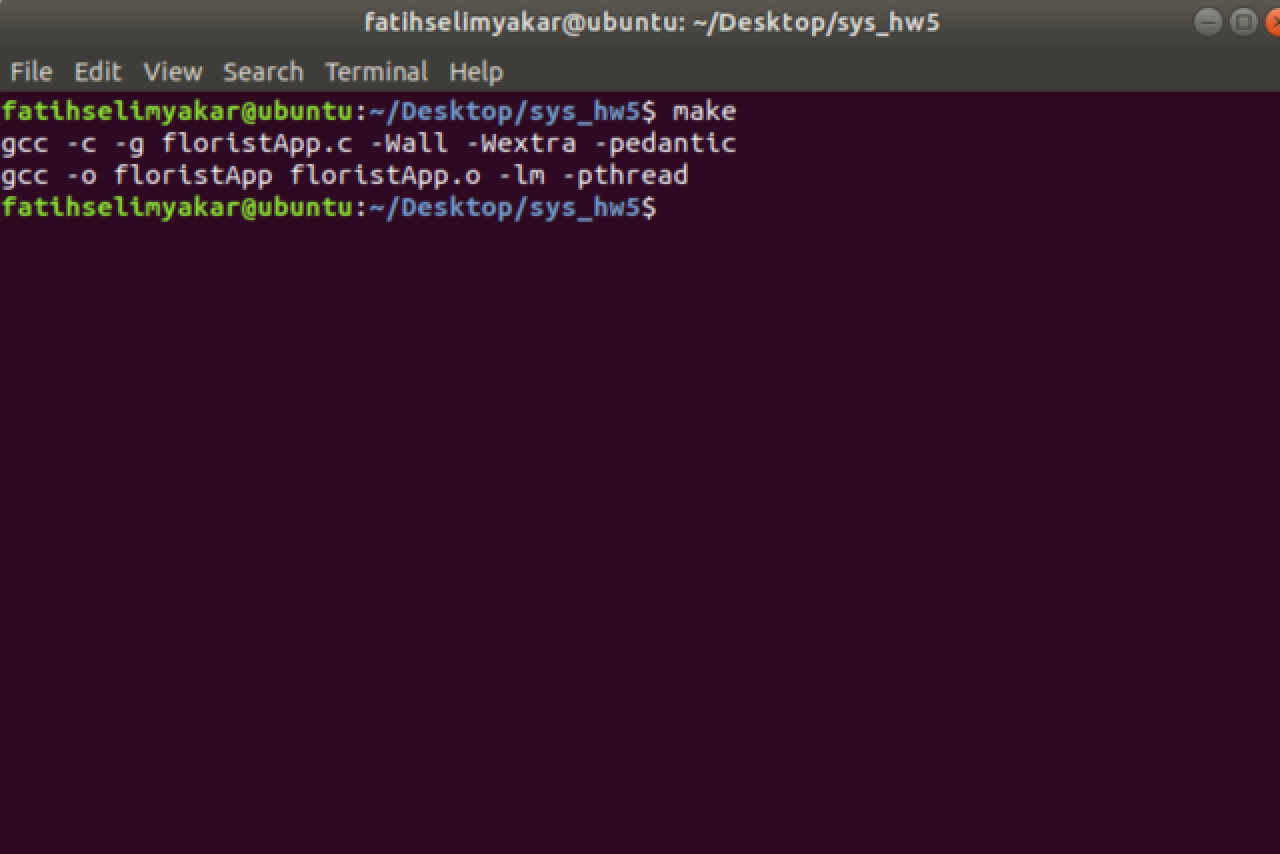
\includegraphics[scale=0.6]{makefile.png} \\[0.5in]
    \textbf{Running result of given "data.dat" with valgrind} \\
    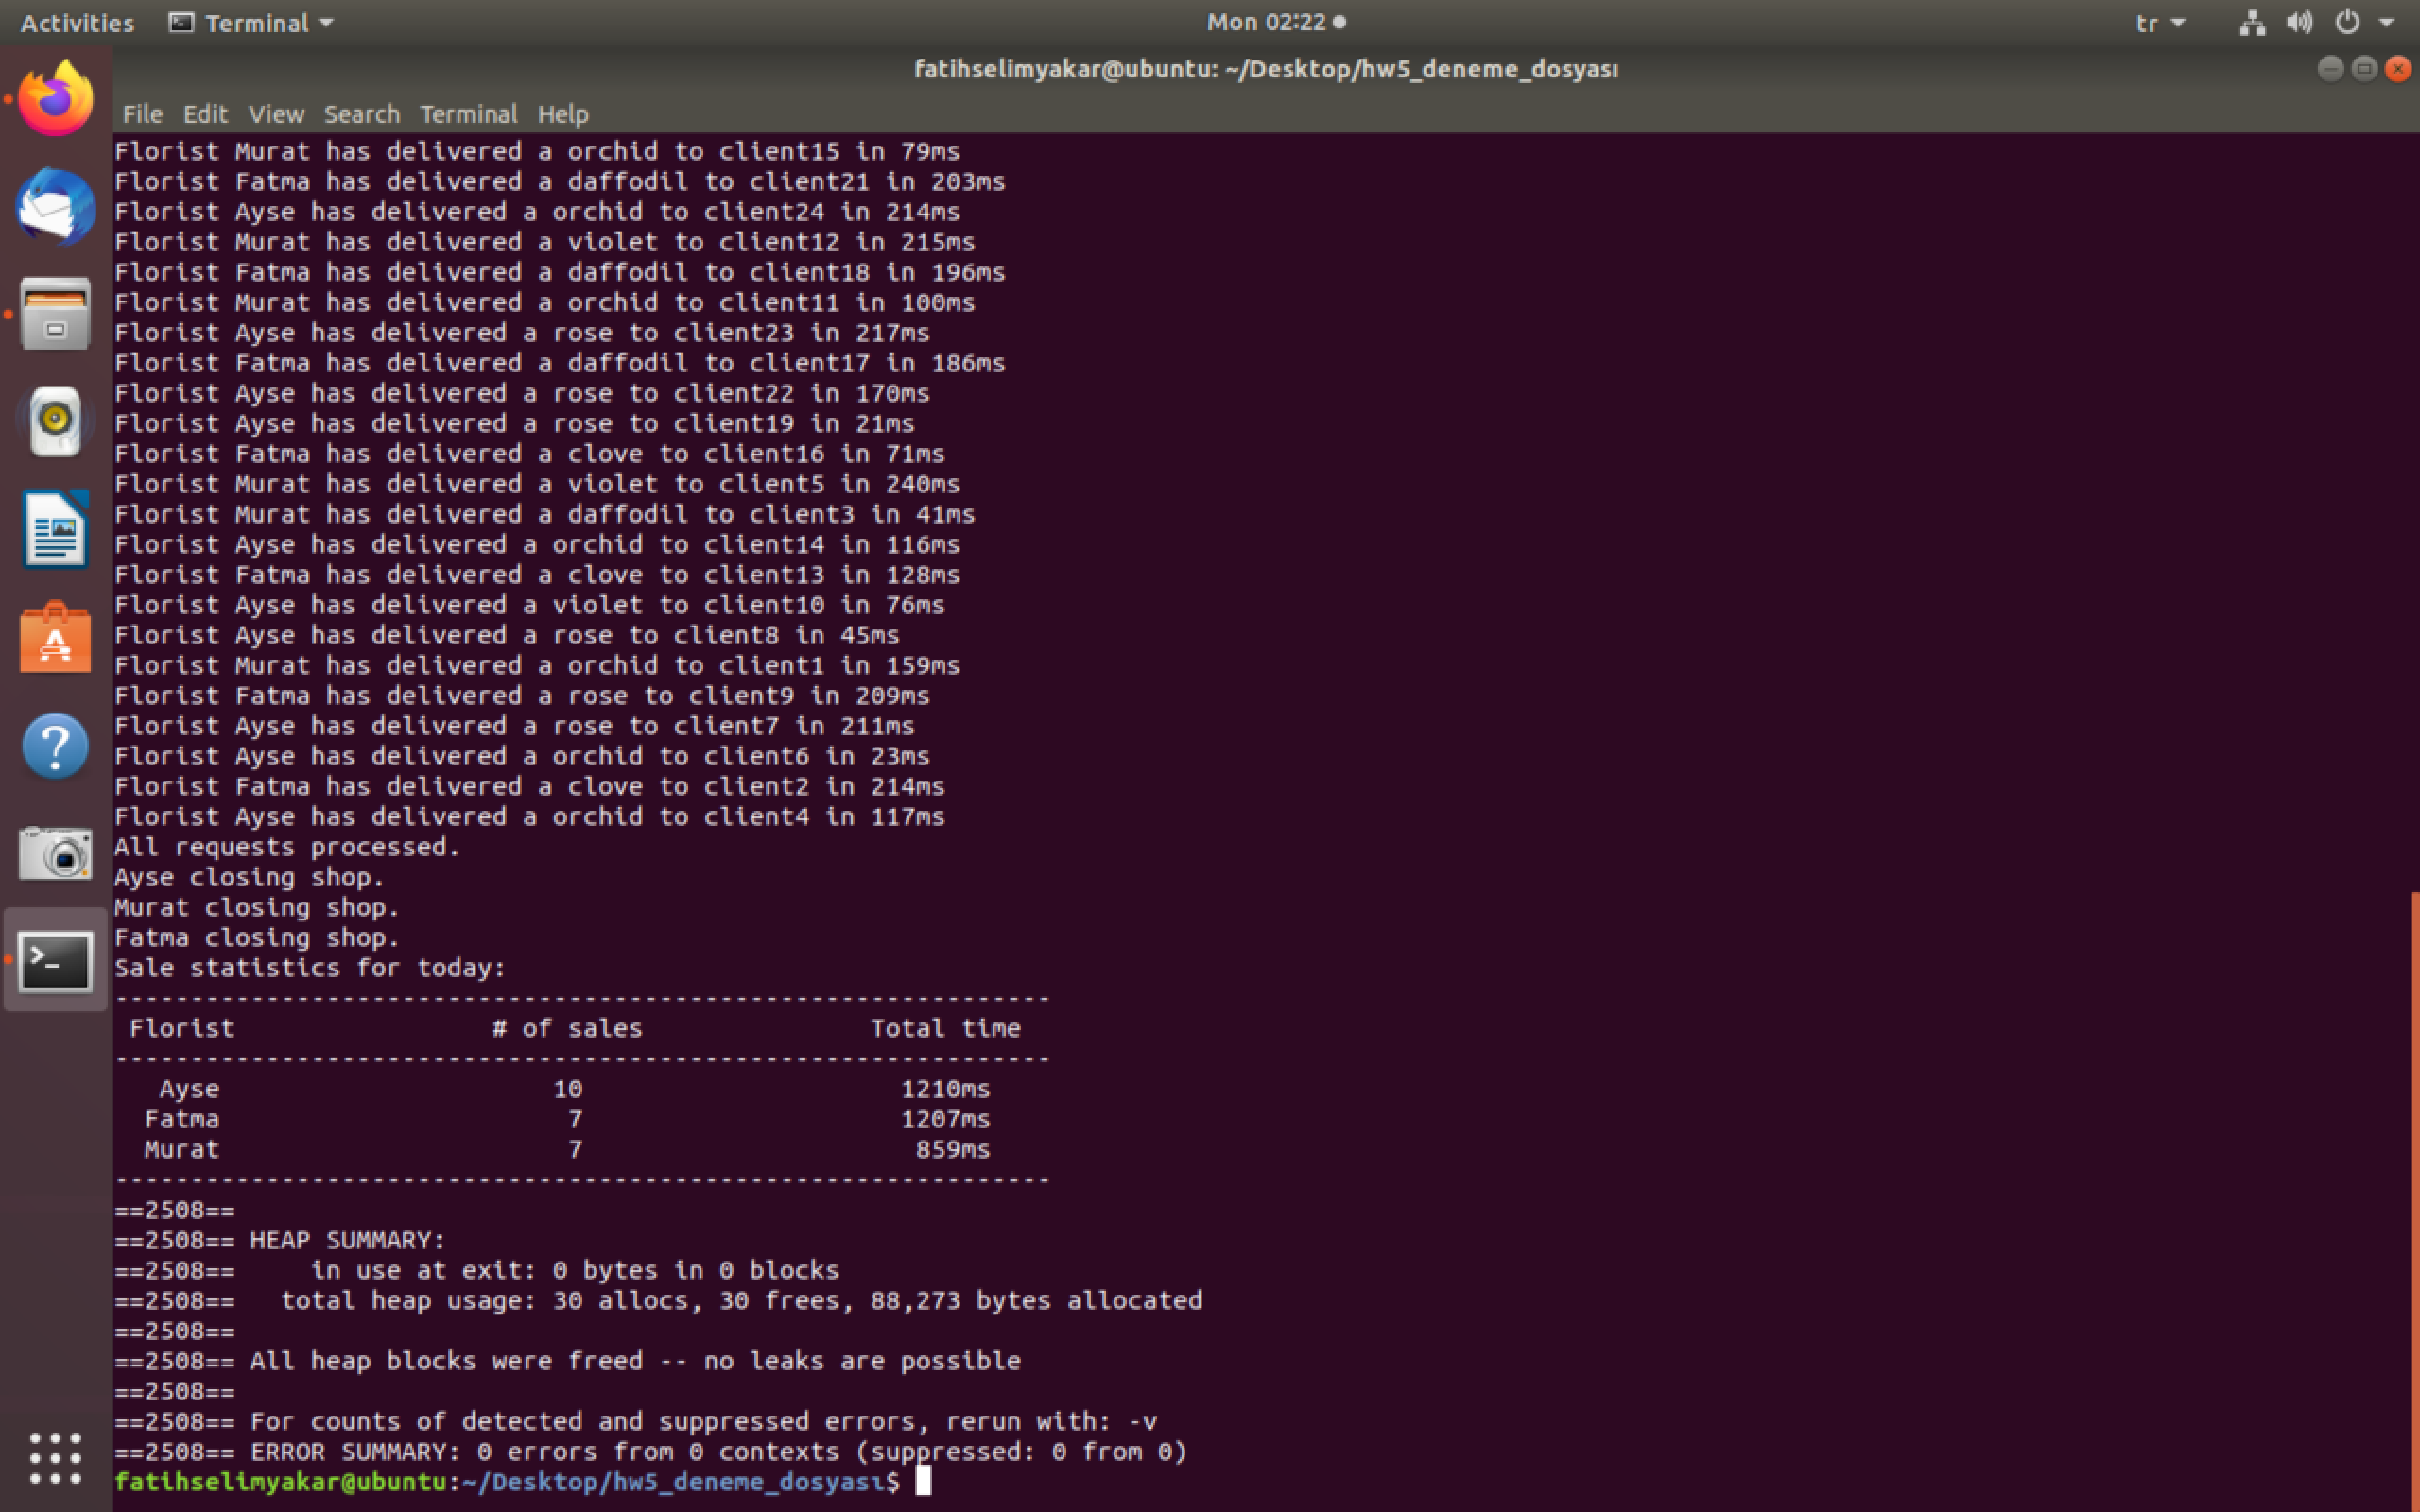
\includegraphics[scale=0.3]{valgrind.png}
    \newpage
    \textbf{In case of CTRL-C} \\
    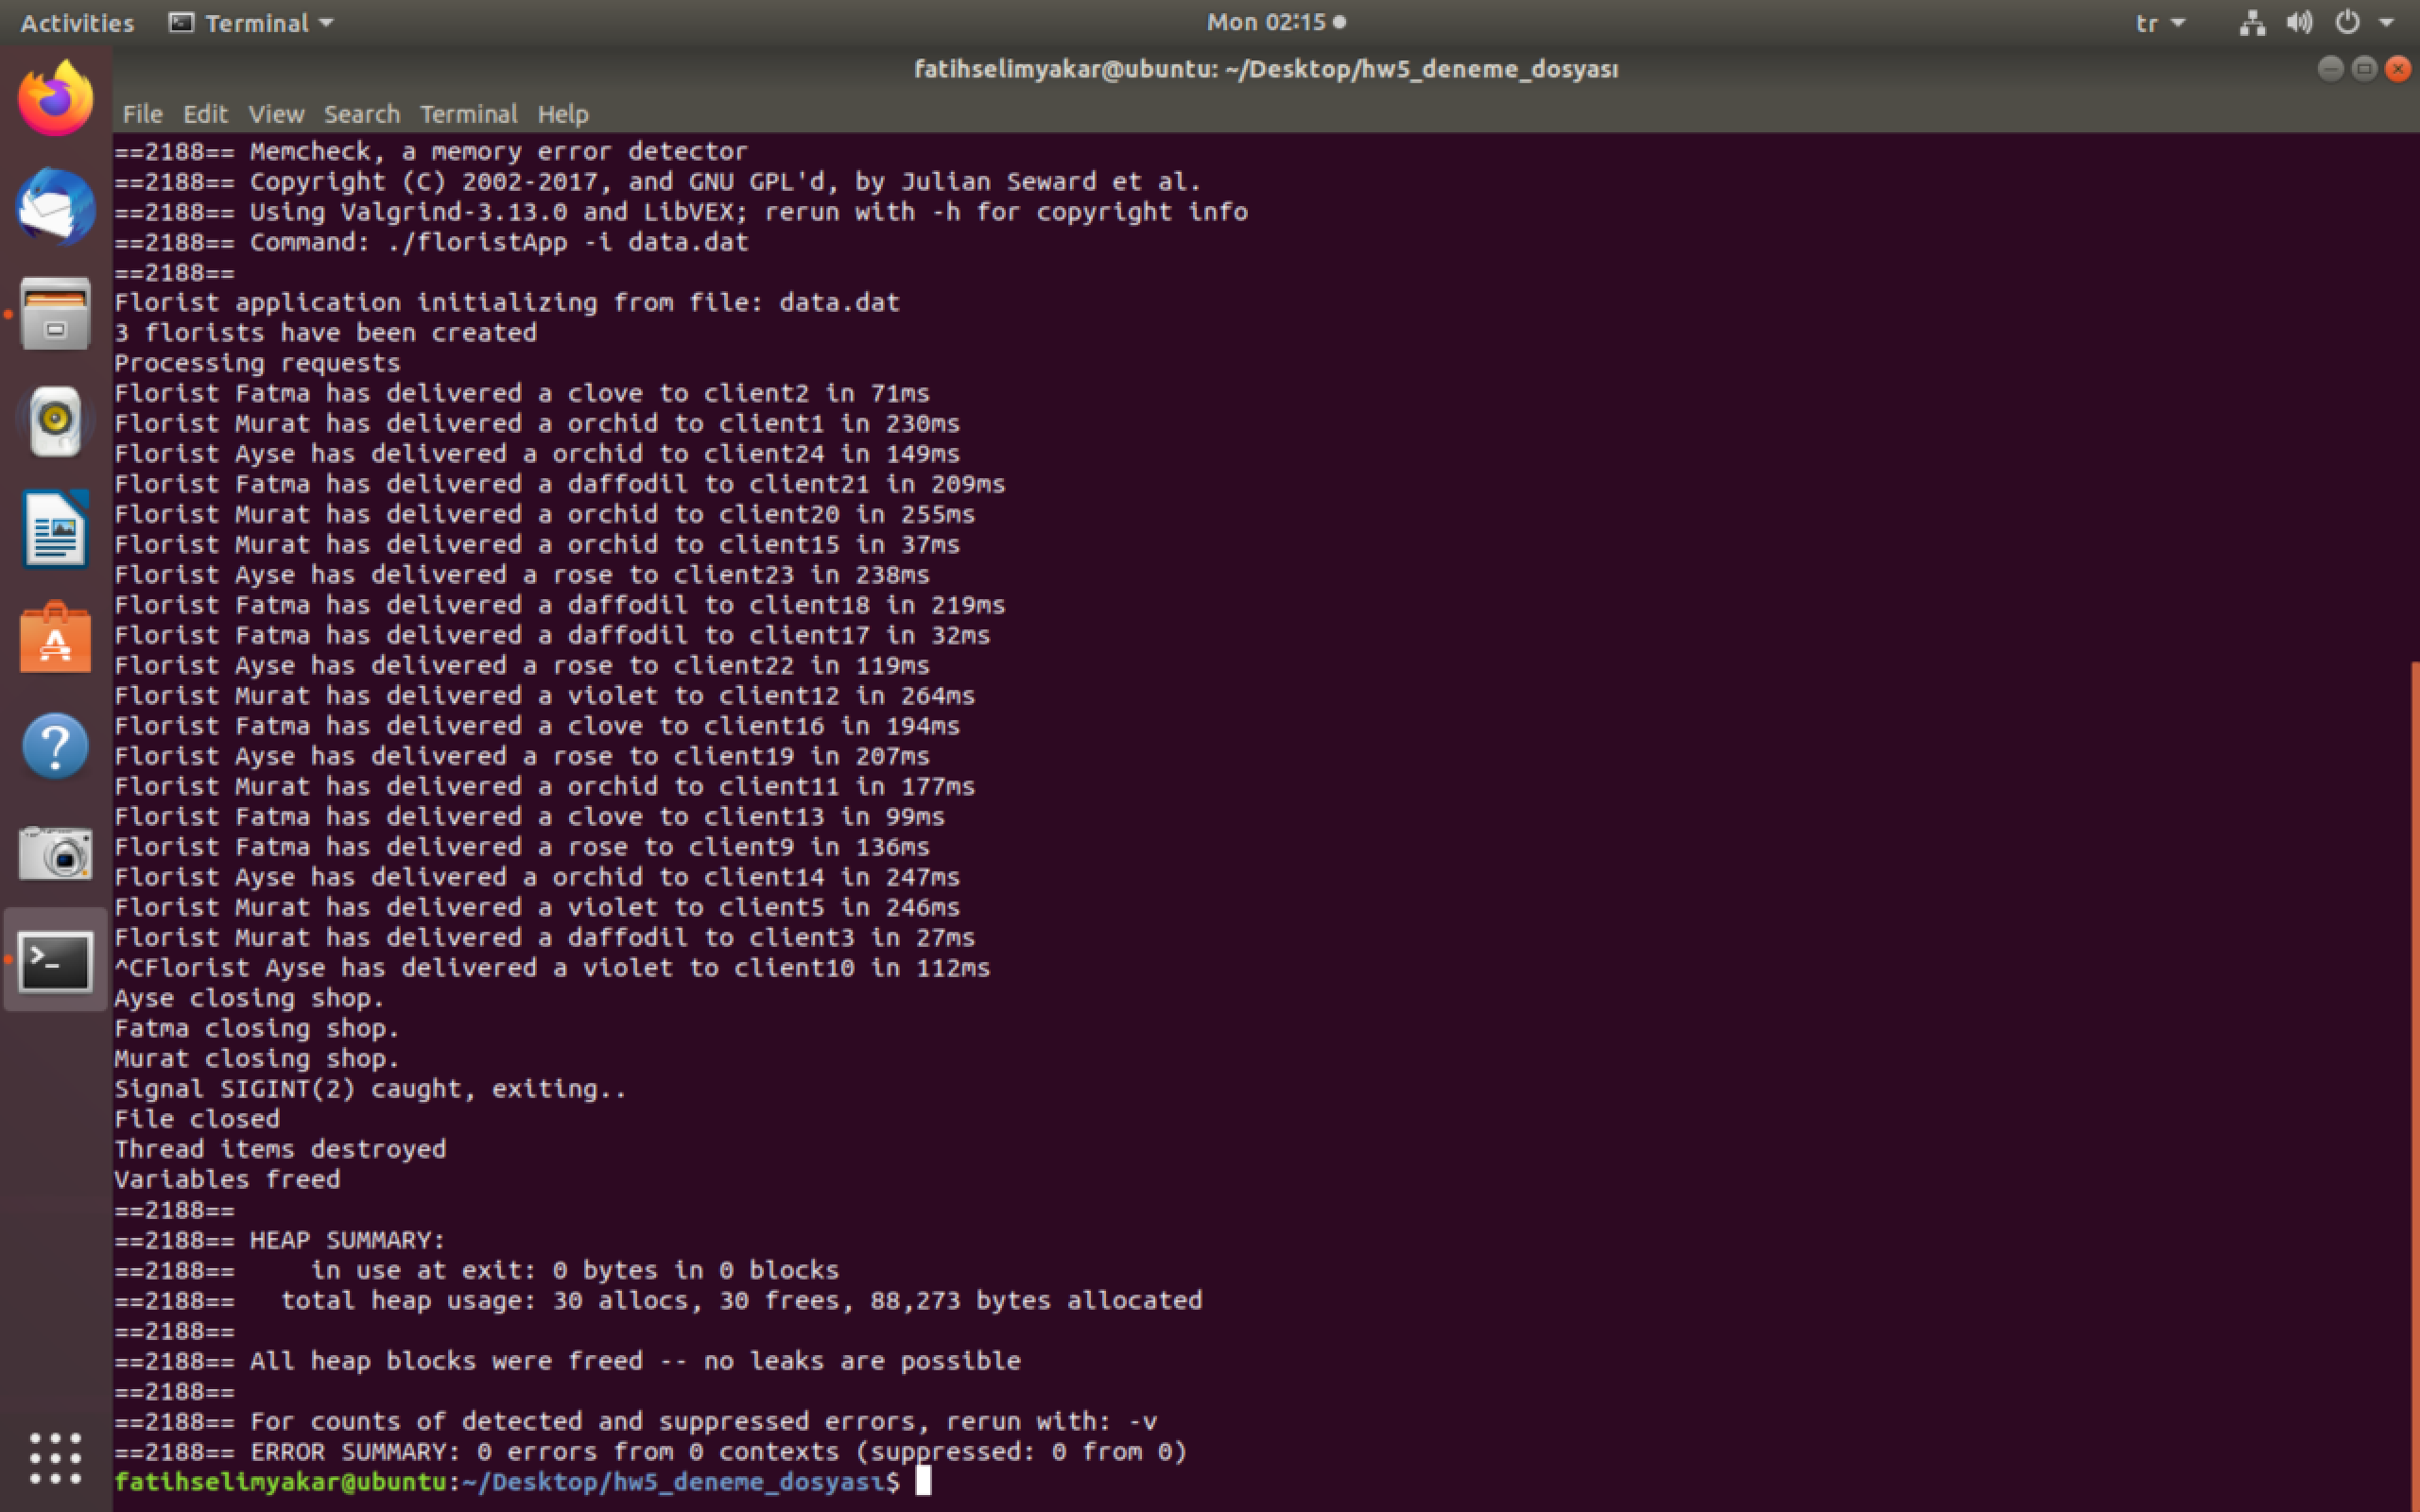
\includegraphics[scale=0.3]{ctrl.png} \\[0.5in]
    \textbf{Fully normal running result} \\
    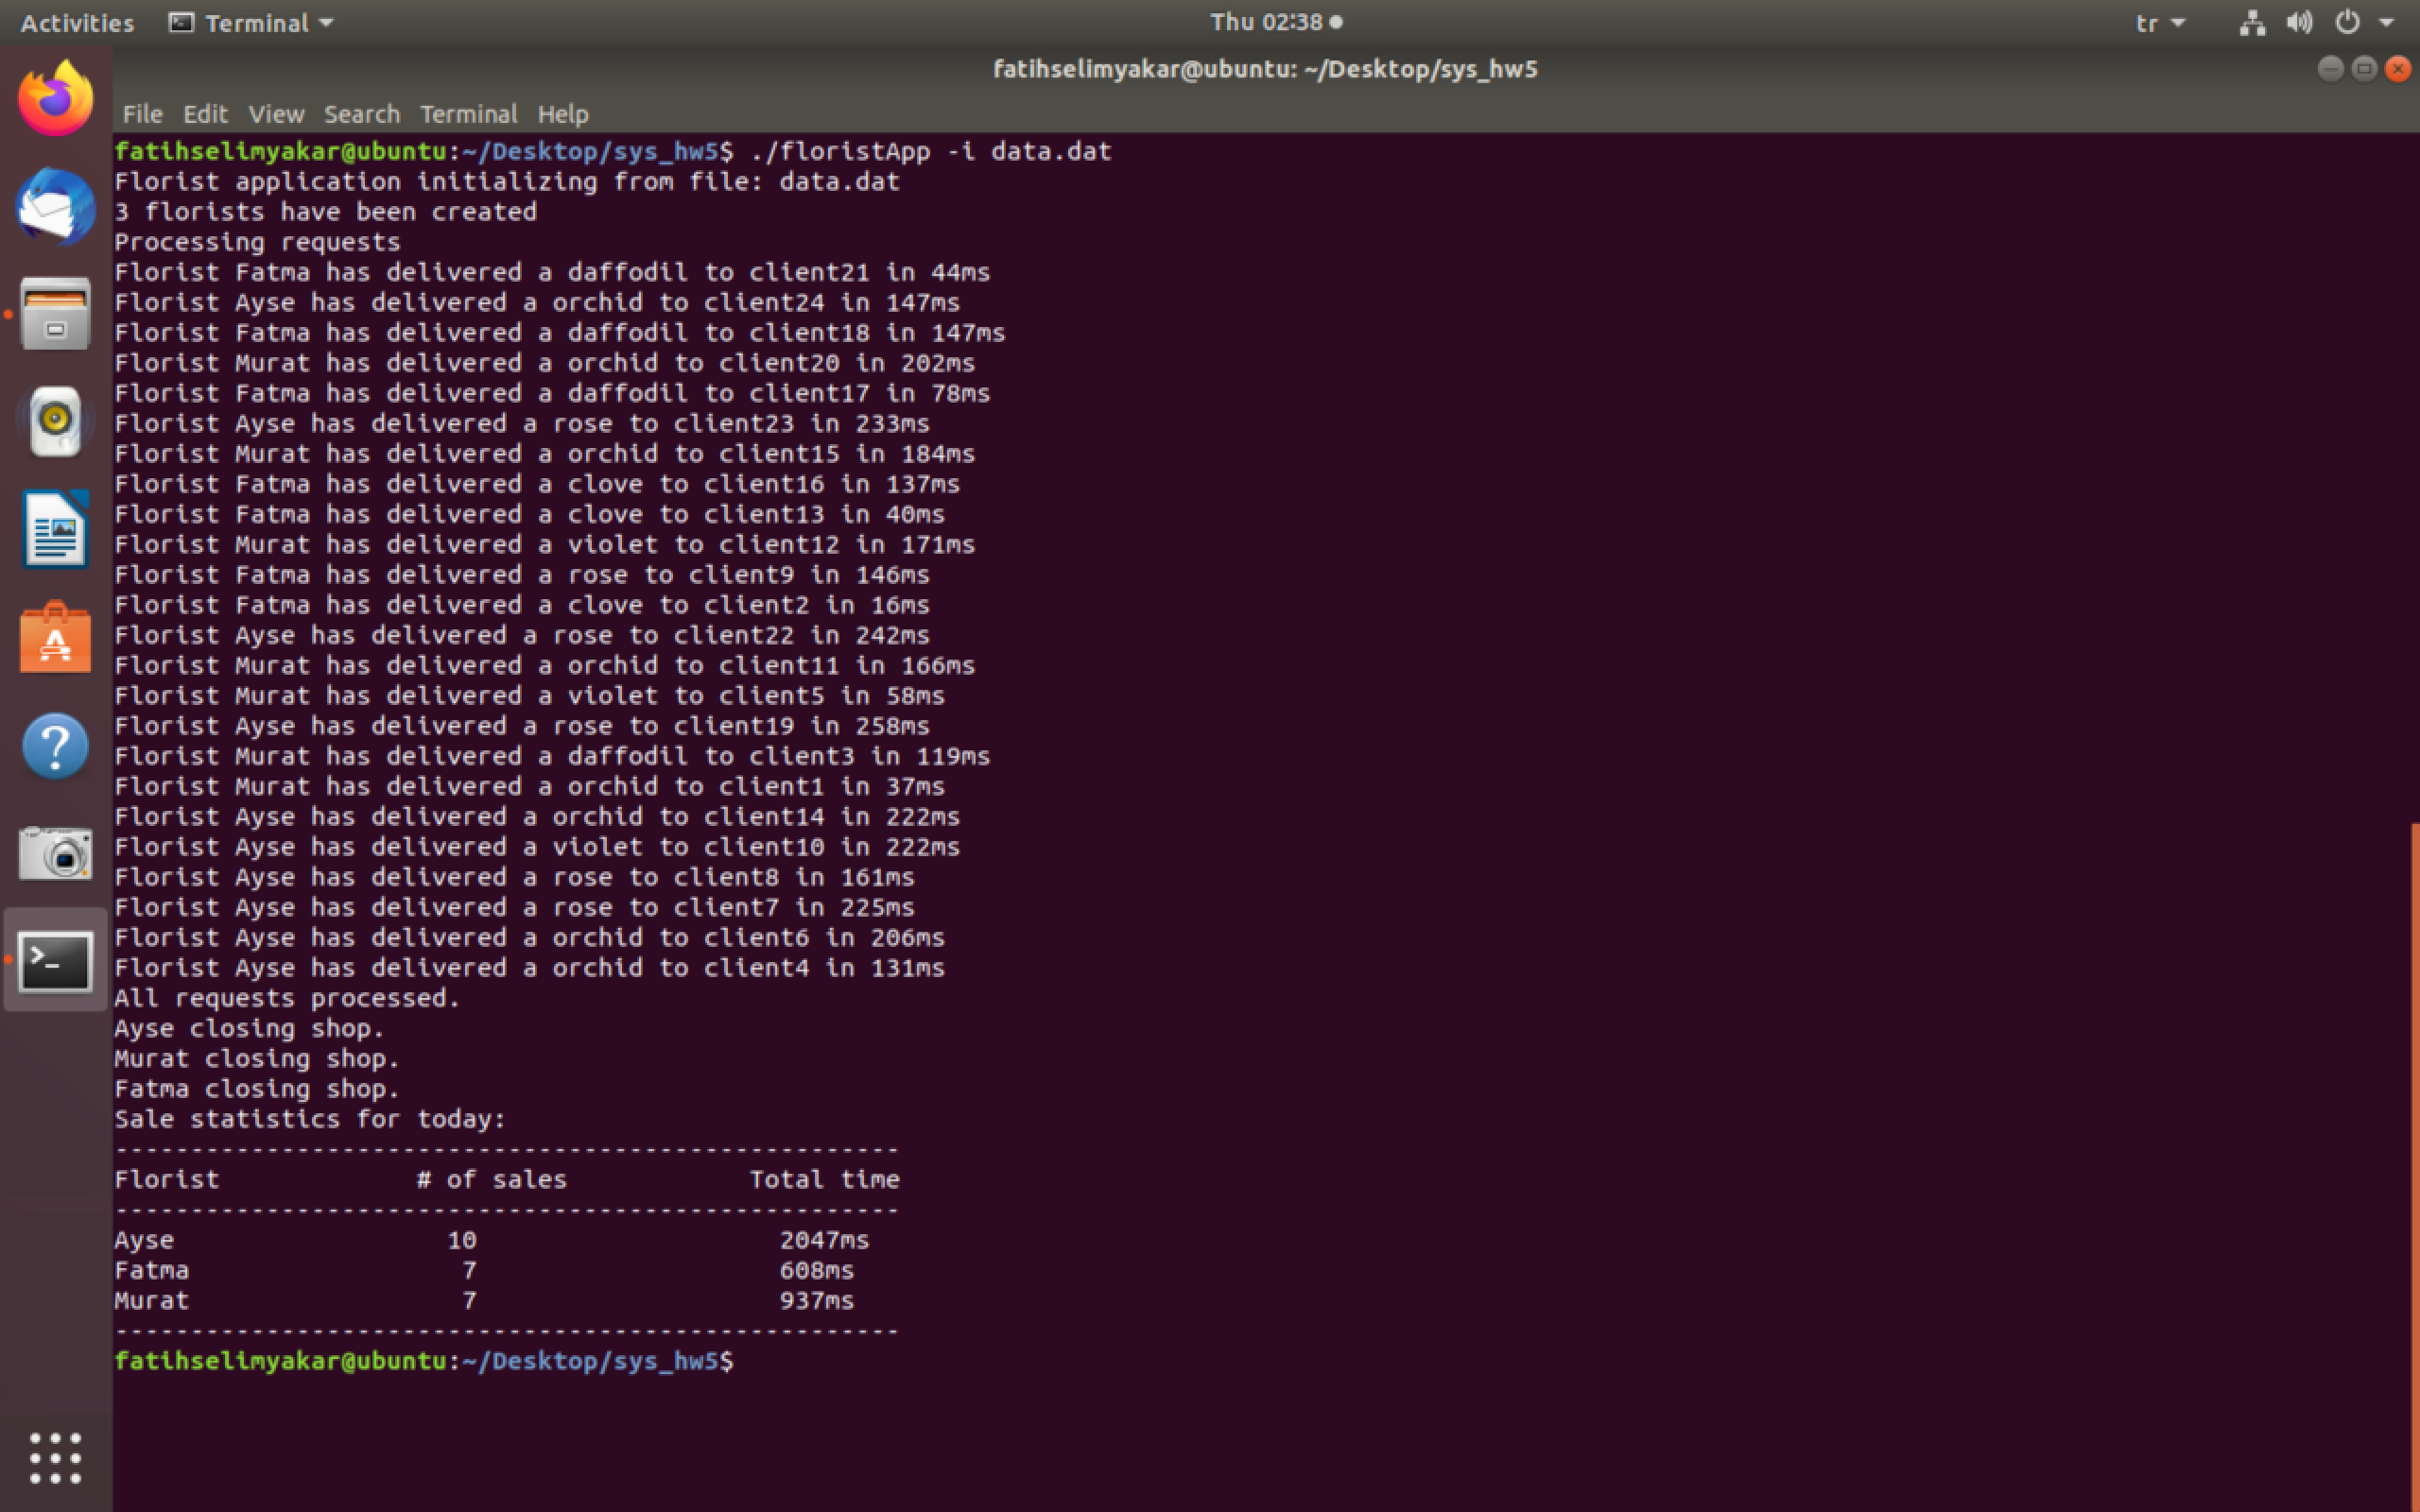
\includegraphics[scale=0.3]{normal.png}
\end{center}
    

\end{document}
